%-------------------------------------------------------------------------------
% jack
%-------------------------------------------------------------------------------
%
% \file        jack.tex
% \library     Documents
% \author      Chris Ahlstrom
% \date        2016-01-28
% \update      2022-11-27
% \version     $Revision$
% \license     $XPC_GPL_LICENSE$
%
%     Provides the JACK page section of seq66-user-manual.tex.
%
%-------------------------------------------------------------------------------

\section{JACK}
\label{sec:jack}

   This section describes some details concerning the JACK support of
   \textsl{Seq66}.
   As with \textsl{Seq24}, \textsl{Seq66} has JACK transport support.
   JACK supposedly works with \textsl{Windows}, but we do not provide a JACK
   MIDI engine for that system at this time.
   The JACK support is very loosely based on the RtMIDI project
   \cite{rtmidi}.
   This mode also supports fallback to ALSA if the JACK server is not running.
   \textsl{However}, if the \texttt{jack-dbus} is running, then a pair of virtual
   ports are created.

   \index{jack!transport}
   To enable the JACK transport support at run-time on
   \textsl{Linux}, the options
   \texttt{-j}/\texttt{-{}-jack-transport} (deprecated, a legacy option),
   \texttt{-S}/\texttt{-{}-jack-slave} (the new version of the transport
   option),
   \texttt{-J}/\texttt{-{}-jack-master},
   and \texttt{-C}/\texttt{-{}-jack-master-cond} are available.
   \texttt{-g}/\texttt{-{}-no-jack-transport}
   disables JACK transport even it JACK is running.
   Also see \sectionref{subsubsec:configuration_rc_jack_transport}.

   Note that the JACK transport options are \textsl{separate} from JACK MIDI.
   \index{jack!midi}
   To enable JACK MIDI, the options \texttt{-t}, \texttt{-{}-jack-midi},
   and \texttt{--jack} are available.
   Note that the \texttt{--jack-midi} and \texttt{--jack} options both
   enable JACK MIDI.

   If one wants to use \textsl{Seq66} and USB devices
   with JACK MIDI, one needs to expose the USB ports to JACK using the
   command \texttt{a2jmidid -{}-export-hw}.

   If \texttt{jackdbus} (Linux) is installed on the system, it is recommended
   to use \texttt{jack\_control} or the wrapper script \texttt{jackctl}
   provided by \textsl{Seq66}.
   The following sections discuss the JACK transport support and the native
   JACK MIDI support.

\subsection{JACK / Transport}
\label{subsec:jack_transport}

   JACK transport support is \textsl{separate} from native JACK MIDI support,
   and uses a separate JACK client.
   The JACK transport client is an invisible client with the
   name "seq66master" or "seq66slave", while the JACK MIDI client is visible in
   \textsl{QJackCtl}, and the ports created are part of the
   "seq66" client.

   \textsl{Seq66} can be configured to run without JACK transport, with JACK
   transport as a "slave" (i.e. "client"), as JACK master, or as JACK master if
   there is no other master detected.
   Transport clients were formerly known as "transport slaves", and that
   term seems more clear than "client".

   The \textsl{timebase master}
   continuously updates extended position information, counting beats,
   timecode, etc., while the transport is rolling.
   There is at most one master active at a time. If no
   timebase master, frame numbers are the only position information available.
   If a new client takes over, the former master timebase is no longer used.
   Taking over the timebase may be done conditionally, in which case the takeover
   fails when there is a master already. The existing master can release it
   voluntarily, if desired.
   There are some playback functions that JACK transport does not address:

   \begin{itemize}
      \item Variable speed playback.
      \item Reverse playback.
      \item Looping.
   \end{itemize}

   As per the rules of JACK, any client can start and stop the transport, and
   the other clients will follow suit.  When \textsl{Seq66} is a JACK client,
   it will accept beats/minute (BPM) changes from another client that is
   running as master.  When \textsl{Seq66} is master, changes to its BPM will
   be transmitted to the other clients.

   \textbf{Rules of JACK Transport}:

   \begin{itemize}
      \item Any client can be master, no need for one master client.
      \item Multiple clients can change the transport state;
         any client can start/stop playback or seek to a new location.
      \item The transport timebase (tempo) is set and maintained by
         one of the clients.
   \end{itemize}

   Here are some test JACK Transport scenarios using
   \textsl{Seq66} and \textsl{Hydrogen} running under JACK.
   We currently have to restart Seq66 between each scenario.

   \textsl{Seq66 as JACK Slave, Hydrogen as JACK Slave}

      Either application can start and stop playback on both applications.
      The BPM (beats-per-minute) are changed independently on each application.

   \textsl{Seq66 as JACK Slave, Hydrogen as JACK Master}

      Either application can start and stop playback on both applications.
      Changing BPM on Hydrogen also changes it on Seq66, but not the other way
      around. Seq66 cannot change its BPM via the user-interface.

   \textsl{Seq66 as JACK Master, Hydrogen as JACK Slave}

      Either application can start and stop playback on both applications.
      Changing BPM on Seq66 also changes it on Hydrogen.  If changed on Hydrogen,
      the BPM immediately returns to Seq66's BPM.

   \textsl{Seq66 as JACK Master, Hydrogen as JACK Master}

      If Hydrogen is already running, as soon as Seq66 starts, Hydrogren
      relinquishes JACK Master.
      If Hydrogen comes up after Seq66, it retains JACK Master status.  Both
      applications can control start/stop and BPM

   Note that, in \textsl{Seq66}, a changed BPM resets to the file-value after
   restart.  Bug or feature?

\subsection{JACK / Native MIDI}
\label{subsec:jack_native_midi}

   Currently, \textsl{Seq66} will connect to a JACK
   client automatically only at startup, where it will connect to all JACK
   clients that it finds.  If it can't find a JACK client, then it will
   fail to register a JACK port, and cannot play.

   The other option is to set up virtual ports using the
   \texttt{-{}-manual-ports} or \texttt{-{}-options virtual=o,i} options, and then
   to manually connected these ports to the desired MIDI devices or
   applications using \textsl{QJackCtl} (for example).

   To run with JACK MIDI, just make sure JACK is running, then start
   \textsl{Seq66}, which will detect JACK and use it.
   If it instead opts to run with ALSA, edit the 'rc' file to set up
   \texttt{midi\_jack}, or add the
   \texttt{-t}, \texttt{-{}-jack-midi},
   \texttt{-{}-jack}
   or option to the command-line.
   If \textsl{Seq66} doesn't find JACK, it will fall back to ALSA.

	\index{sticky options}
   The JACK (\texttt{-t}) and ALSA (\texttt{-A}) options are sticky options.
   That is, they are saved to the 'rc' configuration file at exit,
   so one does not have to specify them in subsequent \textsl{seq66} sessions.

\subsubsection{JACK / MIDI Output}
\label{subsubsec:jack_midi_output}

   By default (or depending on the 'rc' configuration file),
   \textsl{Seq66} will
   \index{jack!auto-connect}
   \index{auto-connect}
   automatically connect the ports that it finds to \texttt{seq66}.
   The following figure shows connections to a number of USB MIDI devices
   (purple) that have been bridged to JACK (red) by the \texttt{a2jmidid}
   daemon.

\begin{figure}[H]
   \centering 
   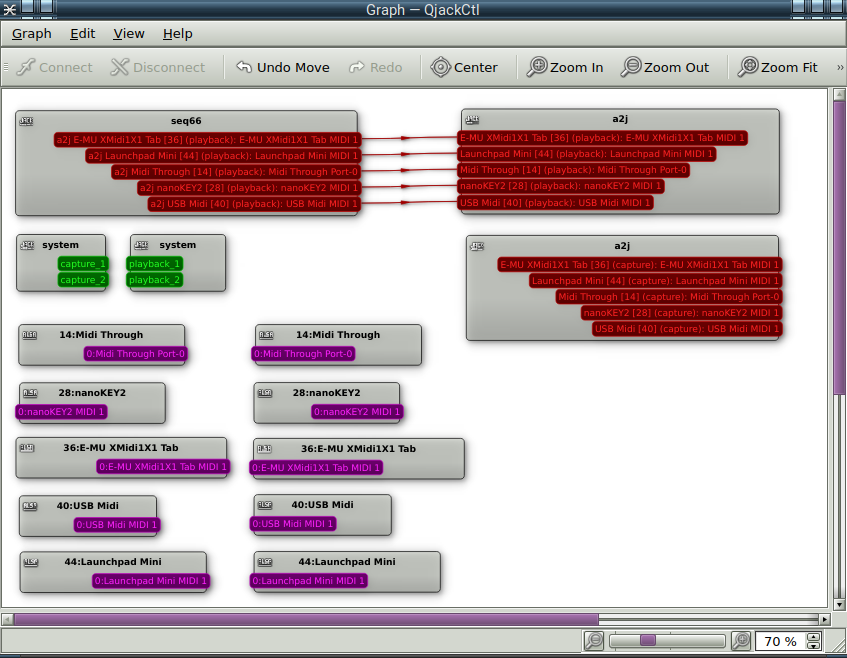
\includegraphics[scale=0.40]{jack/qjackctl-a2j-graph.png}
   \caption{JACK MIDI Ports and Auto-Connect}
   \label{fig:jack_midi_ports_auto_connect}
\end{figure}

   Note that the ports in \textsl{Seq66} are named after the devices to which
   they are connected.
	The output ports available are shown in \textsl{seq66}'s
	\textbf{Edit / Preferences / MIDI Clock} tab.
   If USB devices are not shown, that means
   that the \texttt{a2jmidid} is not running.
   There is a \texttt{bash} script, \texttt{data/linux/startjack}
   that will run \texttt{jack\_control} and \texttt{a2j\_control} to start JACK
   and the \texttt{a2jmidid} daemon to provide full support.
   On our current setup, it creates devices with long names (abbreviated inside
   \textsl{Seq66}):

   \begin{verbatim}
6    # number of MIDI clocks (output busses)
 0 0 "[0] 0:0 seq66:a2j Midi Through [14] (playback): Midi Through Port-0"
 1 0 "[1] 0:1 seq66:a2j Launchpad Mini [28] (playback): Launchpad Mini MIDI 1"
 2 0 "[2] 0:2 seq66:a2j E-MU XMidi1X1 Tab [32] (playback): E-MU ... Tab MIDI 1"
 3 0 "[3] 0:3 seq66:a2j nanoKEY2 [36] (playback): nanoKEY2 MIDI 1"
 4 0 "[4] 0:4 seq66:a2j USB Midi [40] (playback): USB Midi MIDI 1"
 5 0 "[5] 1:5 seq66:yoshimi-01 midi in"
   \end{verbatim}

   A feature new with version 0.98.5 is that an output port can be enabled or
   disabled in the 
	\textbf{Edit / Preferences / MIDI Clock} tab,
   and the change in status takes effect immediately.
   One minor issue is that, upon reenabling, a stray note or two might be
   emiited.

\subsubsection{JACK / MIDI Input}
\label{subsubsec:jack_midi_input}

   The input ports also end up with long names:

   \begin{verbatim}
5   # number of input MIDI busses
0 1 "[0] 0:0 seq66:a2j Midi Through [14] (capture): Midi Through Port-0"
1 1 "[1] 0:1 seq66:a2j Launchpad Mini [28] (capture): Launchpad Mini MIDI 1"
2 1 "[2] 0:2 seq66:a2j E-MU XMidi1X1 Tab [32] (capture): E-MU ... Tab MIDI 1"
3 0 "[3] 0:3 a2j:nanoKEY2 [36] (capture): nanoKEY2 MIDI 1"
4 0 "[4] 0:4 a2j:USB Midi [40] (capture): USB Midi MIDI 1"
   \end{verbatim}

   When the check-box for a buss is selected, that input can be captured by
   \texttt{seq66}.
   An output port can be enabled or disabled in the 
	\textbf{Edit / Preferences / MIDI Input} tab.

\subsubsection{JACK / MIDI Virtual Ports}
\label{subsubsec:jack_midi_virtual_ports}

   \index{ports!manual}
   \index{ports!virtual}
   The manual-versus-normal port support for JACK MIDI is essentially the same
   as that for ALSA.
   The \texttt{-{}-manual-ports} and
   \texttt{-{}-options virtual=o,i} options provide
   "virtual ports".  These are ports that do not represent
   hardware, but are created by applications to allow them to connect to other
   applications or MIDI devices.

   The difference between manual/virtual ports and normal ports is that, while
   normal ports are automatically connected to the remote ports that exist in
   the system, the manual/virtual ports are just created, and one must
   manually connect them via, for example, the
   \textsl{QJackCtl} connections dialog.

   So, if one wants \textsl{seq66} to automatically connect to all existing
   JACK MIDI ports, \textsl{do not} use the
   \texttt{-m}/\texttt{-{}-manual-ports} option... use the
   \texttt{-a}/\texttt{-{}-auto-ports} option.  Both options apply to both
   ALSA and JACK.
   The \textbf{MIDI Clock} and \textbf{MIDI Input} tabs reflect
   what is seen in \textsl{QJackCtl}.

\subsubsection{JACK / MIDI and a2jmidid}
\label{subsubsec:jack_midi_a2jmidid}

   One thing we saw is that \texttt{seq66} can deal with the odd naming
   of JACK ports created by the \textsl{a2jmidid} application.
   One can see in the input and output lists shown earlier
   that that the \texttt{a2j} client creates entries for "Midi Through",
   software clients, and bridged USB MIDI devices.
   Again, if these automatic connections get in the way, run \texttt{seq66} in
   manual/virtual mode.

   To set up \textsl{JACK}, one can use the script shipped with
   \textsl{Seq66}, \texttt{data/linus/startjack}.  It has the following
   requirements and dependencies:

   \begin{itemize}
      \item \texttt{qjackctl}.  Provides a way to show the connections. It also
         can start \textsl{JACK}, but we use \texttt{jack\_control} for that in
         this script.
      \item \texttt{jack\_control}.  Provides a way to start \textsl{JACK}
         and set up a number of \textsl{JACK} parameters.
         Part of the \textsl{Debian} \texttt{jack2d} package.
      \item \texttt{a2j\_control}.  Provides a way to configure and start the
         \textsl{ALSA}-to-\textsl{JACK} bridge to create bridges for all the
         hardware MIDI ports on the computer.
         Part of the \textsl{Debian} \texttt{a2jmidid} package.
      \item \texttt{yoshimi}.  Provides a software synthesizer for MIDI
         playback.
      \item \texttt{yoshimi-b4uacuse-gm.state}.  Provides a "General MIDI"
      setup for \textsl{yoshimi}.  Located in the \texttt{data/linux}
      directory.
      \item \textsl{Editing}.  One must edit the script to change the value of
      \texttt{HWPORT}
   \end{itemize}

   One can also edit the script to use another software synthesizer.
   Once ready, 
   Run \texttt{startjack} and wait patiently for it to set up.

\subsection{JACK / Trouble-Shooting}
\label{subsec:jack_testing}

   This section describes some trouble-shooting that can be done with JACK.

\subsubsection{JACK / Trouble-Shooting / MIDI Clock}
\label{subsubsec:jack_testing_midi_clock}

   There are three common timecode formats: LTC (Linear Time Code),
   MTC (MIDI Time Code), and MIDI Clock, as well
   as JACK transport.
   This section describes MIDI Clock.
   It is an alternative to using JACK transport to synchronize devices.

   MIDI Clock is not a timecode format but tempo-based time. The absolute
   reference point is expressed as beats-per-minute and bar:beat:tick.
   There is no concept of sample-locking for MIDI clock signals.

\paragraph{JACK MIDI Clock Send}
\label{paragraph:jack_testing_midi_clock_send}

   To verify that \textsl{Seq66} is sending MIDI clock, the easiest way (using
   JACK) is to start the following command and set \textsl{Seq66} to send
   MIDI Clock to the \texttt{jack\_mclk\_dump} port
   that appears after restarting
   \textsl{Seq66}:

   \begin{verbatim}
      $ jack_mclk_dump
   \end{verbatim}

   Once set up, start playback on \textsl{Seq66}.
   The result should be a 0xfa (MIDI Start) message,
   a never-ending stream of rapid MIDI clock messages,
   and then, upon stopping playback, a 0xfc (MIDI Stop) message.

   Do not try to use \textsl{gmidimonitor}... while it displays Start and Stop,
   it does not display MIDI Clock.

\paragraph{JACK MIDI Clock Receive}
\label{paragraph:jack_testing_midi_clock_receive}

   To verify that \textsl{Seq66} receives MIDI clock in JACK, use a program
   that can emit MIDI Clock in JACK.
   We've tried \texttt{jack\_midi\_clock} to generate time code, but
   it didn't seem to work, even when connected to the
   application \texttt{jack\_mclk\_dump} used in the previous section.
   However, since we verified that \textsl{Seq66} can send MIDI Clock, we can
   use it to test itself.

   First, run the following command using \textsl{debug version of Seq66}, so
   that we can see if it is receiving:

   \begin{verbatim}
      $ qseq66 --jack-midi --manual --verbose --client-name seq66debug
   \end{verbatim}

   This creates virtual JACK ports that show up in a JACK patchbay as part of
   an application called "seq66debug".  This lets us distinguish it from
   the regular version.  Run the following \textsl{Seq66} command:

   \begin{verbatim}
      $ qseq66 --jack-midi --manual --verbose
   \end{verbatim}

   Set MIDI Clock for "midi out 0" to "On" so that it will emit clocking.
   Restart \texttt{qseq66}.
   Then connect the "midi out" of "seq66" to the "midi in" of "seq66debug"
   in the JACK patchbay.
   Then start playback.
   \textsl{seq66debug} should display a rapid stream of MIDI Clock messages.
   If not, check the setup and, if correct, report a bug!

   Note that the \texttt{--jack-midi} and \texttt{--jack} options both
   enable JACK MIDI.

\subsubsection{JACK / Trouble-Shooting / JACK Ports}
\label{subsubsec:jack_trouble_shooting_jack_ports}

   As noted in
   \sectionref{subsubsec:jack_midi_output}, and
   \sectionref{subsubsec:jack_midi_input},
   \texttt{a2jmidid -{}-export-hw} can be used to bridge USB MIDI
   hardware to JACK.  However, on some systems, this bridge can be
   avoided, at the expense of a little confusion.
   For example, look at this partial output of the \texttt{jack\_lsp}
   command:

   \begin{verbatim}
      system:midi_playback_1
      system:midi_capture_2
      system:midi_playback_2
      system:midi_capture_3
      system:midi_playback_3
      system:midi_capture_4
      system:midi_playback_4
      fluidsynth-midi:midi_00
   \end{verbatim}

   The "system" ports correspond to real MIDI devices on this system, but which
   ones?  To find out, run \texttt{jack\_lsp --aliases}.  Here is just one
   device output:

   \begin{verbatim}
   system:midi_capture_2
      alsa_pcm:Launchpad-Mini/midi_playback_1
      Launchpad-Mini:midi/playback_1
   system:midi_playback_2
      alsa_pcm:Launchpad-Mini/midi_capture_1
      Launchpad-Mini:midi/capture_1
   \end{verbatim}

   So system MIDI device 2 is the \textsl{Launchpad Mini}, and
   will show up in \textsl{Seq66} as an I/O device on port 1.
   (Port 0 is usually the system MIDI Thru port).
   Of course, with this arrangement, port-mapping cannot be used.
   In the future, we may be able to ensure the aliases are always
   present in \textsl{Seq66}.

\subsection{JACK / QJackCtl}
\label{subsec:jack_qjackctl}

   This section is a placeholder for discussion of \textsl{QJackCtl},
   its usage of the (deprecated) \textsl{JACK Session API}, and
   its "patchbay" (see \cite{patchbay}).
   Its a good idea to put "jackd -S" instead of just "jackd" for the server
   path. Running JACK in synchronous mode creates less Xruns in JACK2, which
   is now the default.
   
\subsection{JACK / PulseAudio}
\label{subsec:jack_pulseaudio}

   After years of avoiding \textsl{PulseAudio} assiduously, we found a
   circumstance where we needed it.
   In using \textsl{OBS Studio} to make demonstration videos of \textsl{Seq66},
   we struggled trying to get it to work with either
   \textsl{ALSA} or \textsl{JACK} directly.
   Setting up \textsl{PulseAudio} ended up being fairly easy on our
   \textsl{Debian Sid} system, not too
   cumbersome or intrusive (and also made it easier to use
   \textsl{Bluetooth} earbuds via \textsl{pulseaudio-module-bluetooth}).
   However, when we decided to a system reinstall on our main development
   laptop, we ended up installing \textsl{Ubuntu 20}, and it became a real
   pain.

   \index{pulseaudio}
   This section discusses using \textsl{JACK} with \textsl{PulseAudio}.
   After installing \textsl{PulseAudio} and getting it to work with one's
   system (e.g. working with \textsl{Seq66}, \textsl{mpd},
   \textsl{smplayer} etc. using \textsl{ALSA},
   the next step is to install \textsl{JACK} support.
   In \textsl{Debian}-based systems, install \textsl{pulseaudio-module-jack},
   \textsl{pulseaudio-utils}, and \textsl{pavucontrol}.

   Then, assuming \textsl{qjackctl} is installed (which is useful for using
   \textsl{JACK} session management), then go to its menu
   \textbf{Setup... / Options / Execute script ...} and set up each of the
   "jack" scripts found in \texttt{data/linux/jack/pulseaudio}:

   \begin{itemize}
      \item \textbf{Execute script on Startup}:
         \texttt{/usr/local/bin/jack-pre-start.sh}
      \item \textbf{Execute script after Startup}:
         \texttt{/usr/local/bin/jack-post-start.sh}
      \item \textbf{Execute script on Shutdown}:
         \texttt{/usr/local/bin/jack-pre-stop.sh}
      \item \textbf{Execute script after Shutdown}:
         \texttt{/usr/local/bin/jack-post-stop.sh}
   \end{itemize}

   Other executable locations can be used if desired.
   These steps configure \textsl{qjackctl} to run those commands at
   the appropriate time.
   \textsl{PulseAudio} will recognize (via D-Bus) that \textsl{JACK} started,
   and will route audio to it. When \textsl{JACK} is stopped,
   \textsl{PulseAudio} reverts to normal routing.
   Other \textsl{qjackctl} options from the \textbf{Misc} tab:

   \begin{itemize}
      \item \textbf{Start JACK audio server on application startup}:
         Check-mark it, unless one prefers to use the \textbf{Stop} button.
      \item \textbf{Stop JACK audio server on application exit}:
         Check if available, as desired.
      \item \textbf{Single application instance}:
         Check-mark it.
      \item \textbf{Enable ALSA Sequencer support}:
         Recommended.
      \item \textbf{Enable D-Bus interface}:
         Can leave unchecked.
      \item \textbf{Enable JACK D-Bus interface}:
         Can leave unchecked.
      \item \textbf{Save JACK audio server configuration to}:
         Leave unchecked.  If the \texttt{.jackdrc} file is found, then
         \textsl{QSynth} might try to start JACK itself.
   \end{itemize}

   The following scenario describes what we are seeing on
   \textsl{Ubuntu 20.04.3}; the main anomaly is that playback of
   an application through \textsl{PulseAudio} doesn't resume on its own.
   Let's assume we are running \textsl{mpd} and it is playing tunes via
   \textsl{PulseAudio}.
   Then we start \textsl{QJackctl} configured as above.
   This action will silence \textsl{mpd}, but starting playback again will
   work.
   One can then run \textsl{Seq66} using JACK MIDI and JACK transport.
   Once finish, use \textsl{QJackctl} to stop JACK.
   This will silence \textsl{mpd} again.
   Then we have to restart \textsl{PulseAudio} (e.g. via the
   \texttt{repulse} script supplied in \texttt{data/linux/jack/pulseaudio}).

%-------------------------------------------------------------------------------
% vim: ts=3 sw=3 et ft=tex
%-------------------------------------------------------------------------------
